\chapter{Questions for Spatio-temporal Data} %9430
\label{ch:question}

\section{Current Approaches to Questions}
In order to be able to ask better questions it is necessary to first have an understanding of the limitations of current approach to questioning data. Considering Gathering Time, each of the case studies in the two volumes generally considers basic temporal information such as construction dates. For example, at Windmill Hill an objective of the study was to find the date of construction of the enclosure and its constituent circuits \citep[80]{Whittle:2011kl}. In addition, for Windmill Hill, the study aimed to find the duration of primary use, duration being another question consistently asked throughout the study. These two common types of question come in several forms, the first type, ``what date is x?'' also take the form of ``is x earlier or later than y'' as in order to answer this question the dates of x and y are required, these questions are limited in scope to the date itself. The second type of question is where the primary temporal data is used to create some other value or data, for example, in order to calculate duration it is necessary to first calculate two dates to be able to then determine the duration between them. For both these types of question the focus is on the temporal data, even though for the second type the answer actually comes from some derived data. Finally, there are those questions that engage with some level of archaeological theory. Examples of this type of question would include ``whether the contrast in plan and scale between the inner and outer pairs of circuits indicates diachronic construction'' \citep[219]{Whittle:2011kl}, ``Did the simple stratigraphic sequences at Etton Woodgate and Northborough correspond to shorter use-lives than those reflected in sometimes complex histories of recutting and backfilling at Etton'' \citep[318]{Whittle:2011kl} and ``establish whether any of the dated bones were already old when placed in the monument'' \citep[48]{CAJ:676124}. At first glance such questions seem almost entirely heterogeneous, there is no common format or pattern, they are all fairly specific, asking detailed questions of a site that engage with various theories about the site, and how it was used in the past.

These categories of question are fuzzy and in many ways cumulative, for in order to answer those in the final grouping, we will have to have data that could be used to answer questions of date and duration. The kind of questions examined above are being asked and answered with modern analytical techniques. In many cases the more interesting, theoretical questions do not require a special methodology, they simply require the application of the data from the primary analysis to the task of interpretation. This raises the question of why such questions, that engage with theory, are not asked more routinely?

This is not to suggest that the more rudimentary questions are less important, merely that they are limited in scope. In order to make full use of spatio-temporal data it is necessary to ask questions which really push at the boundaries about what is known of people in the past. These kinds of questions, which engage with archaeological theory, have been described as ones that ``investigate \ldots questions beyond the descriptive''  \citep[51]{Evans:2006fk}. They go beyond simply describing the results of statistical analysis, engaging with a theoretical question, with the ultimate objective of influencing archaeological theory, or to put it another way, re-building the scaffolding required to treat data as evidence \citep{doi:10.1177/0162243916671200}.

What Evans means by this is that we should not be satisfied with the ``how old is x'' kinds of questions, and instead should be focusing on questions that use the data to take us closer to the people being studied. In many respects this is not too far removed from the more narrative speculation often placed at the end of publications, however, these spatio-temporal questions should be being asked more formally and make explicit references to their data. With the finer grained dating evidence now available via bayesian modelling such questions should be supplementing (or replacing) the more mundane ``what date is x'' type questions in the core of research.

Clearly these kinds of questions are already being asked of temporal data. But not frequently enough, and there are few examples of such questions engaging with both spatial and temporal elements of the data. In order to examine kinds of questions that should be being asked of archaeological data, it is necessary to engage with archaeological theory. The following section will examine aspects of temporal theory that could provide inspiration and a framework for asking interesting questions. Temporal theory has been chosen for the focus as all of the temporal concepts could be easily extended to include a spatial component and there is a lack of application of this theory, especially when compared to spatial analysis. This is due to the ready availability of spatial techniques from other fields, which could be applied wholesale to archaeological data. This is in contrast to temporal methods, where techniques from other disciplines are not so applicable and a body of theory has developed without this influence. \citet{Bailey:2007fk} has recognised there is a chicken-and-egg situation here, between temporal analytical techniques and questions to ask, how can one ask questions without knowing what techniques are available? But it is not possible to know what tools are required until the questions have been asked. This thesis will start with the questions, as even if it is not possible to answer them at present, it may become so in the future and because starting with the tools may introduce an unintended bias if they are all developed under the same theoretical framework. 

\section{Temporal Theory}
There are a wide range of different topics that fall under the heading of time in the past, and a variety of authors, taking varied philosophical perspectives have focused on these different topics. In a broad review of the area Lucas splits it into the study of time perception and the study of the temporal structure of past activities, however he argues for a close connection between the two, stating ``Society does not solely perceive time through time-marking systems, but through the very temporality of its practices'' \citet[70]{Lucas:2005fk}. While Lucas acknowledges the study of temporal perception, he sees more benefit in the analysis of temporal structure. The analysis of the temporal structure of activities, or time-consciousness, is broken up by Lucas into social memory and social recollective memory. Where social memory is more near term, within living memory, focused on the reproduction of society. While social recollective memory is concerned with more distant times, the use of ritual to engage with the past \citep[84]{Lucas:2005fk}. This is the focus of \citet{Bradley:2002fk} who splits the temporalities into the distant past, a time concerned with origin myths of a society; the immediate past, which focuses on how people would have been aware of the history of their society; the future,  how monuments were used to shape the memories of the future; and finally how people in the past would have responded to evidence from the past.

Such a perceptual approach to time is criticised by \citet{Bailey:2007fk}, who is concerned that the multiple temporalities studied by Lucas and Bradley are in fact temporalities that exist in our present day society, and that we have no evidence that people in the past had the same awareness of time. In fact, he states ``when archaeologists claim to reveal the subjective experiences of past people, [we have no guarantee] they are doing anything other than imposing their own'' \citep[219]{Bailey:2007fk}. Such an attack appears to cut to the core of the Lucas and Bradley's approach to time consciousness, however it need not be absolutely the case. Take, for example Bradley's idea of the mythical past, this is clearly a subjective temporality we can understand, but Bradley's argument does not necessarily mean that people in the past would have attached the same connotations to the idea of a mythical past that we do today. These are words and phrases to help us understand, and are not necessarily prescriptive of what a mythical past might mean to someone in the past. His argument is perhaps more that the concept of a mythical past is the closest analogy that we have to the temporality he is studying. However, Bailey is making an important point about using our own preconceptions of time to cloud how we view the past, it is somewhat ironic that Lucas is guilty of this, as he attacks chronology for leading to totalizing grand narratives, a modern western view of time \citep[13]{Lucas:2005fk}. 
 
\subsection{Time Perception}
Issues of time perception can be studied directly by looking for evidence of devices used for temporal reckoning, an example of this being the alignment of Neolithic stone monuments in Europe, providing evidence for awareness of periodic events such as the winter solstice \citep[73]{Lucas:2005fk}. While there are clearly potential avenues of research in the field of time perception, it is in some ways quite a limited field of study, the evidence required for a convincing ``proof'' of an awareness of time usually relying on how likely the apparent observance could have occurred by chance. There are also potentially complicated issues of interpretation, for example, solar observances may have a related alignment to other events, such as the midwinter sunset being on the same alignment (but exactly opposite) the midsummer sunrise. Even with clear evidence for an awareness of such events, it is essential to consider the distinction made by Lucas and others between time reckoning and time indication \citep[68]{Lucas:2005fk}. While this is evidence for the reckoning of time, it does not imply some sort of calendar, or system of measuring required for time indication. Presumably, any society that relies on horticulture would have to be aware of the changing seasons in one way or another, for the yearly planting of seeds, harvesting, etc, but they would not necessarily record their passing. It is perhaps this type of ambiguity which leads Lucas to the conclusion ``��it is really when archaeology leaves the realm of trying to recover evidence of time-reckoning and explores more general issues of temporal perception in the past and its relation to social practice that the most rewarding studies are to be found''�� \citep[77]{Lucas:2005fk}. 
 
\subsection{Temporal Society}
There is evidence for the temporal structure of past activities, or time-consciousness, in a range of practices. Lucas defines the concept of social memory as the transmission of knowledge in non-literate societies, \citep[77]{Lucas:2005fk}. He argues that the reproduction of society is largely dependent on repetitive incorporation practices. In addition, where such practices are evident in the archaeological record he states they will convey something of the nature of social memory and cultural transmission simply because they tend to be repetitive and incorporative \citep[78]{Lucas:2005fk}. This is down to the innate temporality of society, as recognised by Bradley, who stated ``Time is part of the process of living in society'' \citep[5]{Bradley:2002fk}. Bradley defines two possible methods for the acquisition of social memory, firstly it might have happened by bodily practices including participations in rituals, ceremonies, social conventions, correct behaviour and appropriate use (and destruction) of material culture \citep[12]{Bradley:2002fk}. Secondly, by the building of monuments designed to perpetuate a particular worldview \citep[12]{Bradley:2002fk}. For Lucas, social memory is studied by the explicit analysis of continuity or repetition of cultural practice over a long period, by examining the nature of the practice and what it implies in terms of social memory, \citep[82]{Lucas:2005fk} this being broadly in line with Bradley's bodily practices.

Closely linked to this is the study of continuity (through social memory) or the lack of it. It could suggest conservatism as opposed to innovation, in this case, it would be valid to ask what is the motivation behind a display of continuity? The decision to stick with a conventional form is a conscious one, this decision can tell us just as much about a society as the decision to change forms, as Bradley notes ``people did not make artefacts or build structures according to a traditional format because they were unable to think of anything else. Rather, they did so as a way of adhering to tradition and maintaining links with what they knew of their past'' \citep[11]{Bradley:2002fk}. Lucas suggests it may be used to create a sense of continuity with the past \citep[83]{Lucas:2005fk}. However, if the reverse is shown, i.e. rapid change, this could be an attempt to show a forward looking practice, or a break with the past, ``changes in its [material cultures] character may not have arisen by chance and could actually have resulted from a deliberate attempt to emphasise similarities or contrasts with tradition'' \citet[12]{Bradley:2002fk}. While it may be tempting to apply such a classification broadly, Lucas warns against classifying a whole society in this way, instead he emphasises the importance of looking at particular practices \citet[83]{Lucas:2005fk}.

\subsection{The Past in the Past}
The investigation of how people in the past would have dealt with the past, either of their own society, or the interpretation of evidence of other societies provides a wide scope for study. Lucas calls this social recollective memory, and states that ``it is here that a society's own sense of time will be most evident as the use of ceremonies and material culture is a dominant part of social recollection, through ritual practices which intentionally engage with the past'' \citep[84]{Lucas:2005fk}. Engagement with the past is a key part of this for Lucas, to study this theme he recommends: \begin{quote}``any aspect of the archaeological record that would seem to indicate some reference to an earlier part of that record might be interpreted in this way. For example re-use of old monuments, the curation and re-use of artefacts, even imitation `old' material culture, suggests that some explicit reference is being made to the past'' \citep[84]{Lucas:2005fk}.\end{quote} However, the study of the collective memory of a society in some ways has parallels to a historical document, in that it is not necessary a straightforward statement of fact. Collective memory can be used as a tool of power by elites who exploit traces of the past in order to make a connection with the status quo in their present, providing an authority drawing on the collective memory of the population \citep[88]{Lucas:2005fk} with the inverse of this being the destruction of traces of the past in order to sever any material links with it \citep[88]{Lucas:2005fk}. And it is not just monuments whose re-use can be examined to provide insights into issues of social memory, Lucas argues that the same notions apply just as much to the re-use of artefacts \citep[89]{Lucas:2005fk}. The study of how a society engages with its past is often conducted on a per monument basis as a biographical review of a monument's life \citep[or lives,][14]{eps376489} and recent examples would include \citet{Guardaino2015,Hvass2015}, with the avenue of research ultimately tracing its way back to \citet{10.2307/125007,Holtorf:2000fk,Bradley:2002fk} although depending on the particular approach taken, additional influences often include biography of objects or literary analysis, such as, e.g. \citet{doi:10.1080/00438243.1999.9980439}.

In many ways this is similar to Bailey's ``Palimpsest of Meaning'', \citep{Bailey:2007fk} which he defines as ``the succession of meanings acquired by a particular object, or group of objects, as a result of the different uses, contexts of use and associations to which they have been exposed'' \citep[208]{Bailey:2007fk}. This could apply just as much to monuments or landscapes and these meanings could include peoples' perceptions of what these monuments were in the past. According to Bailey, these stratified meanings can be interpreted by looking at the physical changes that have been made, as these will be indicative of the change to meaning. Such modifications are problematic however as they can remove some of the characteristics that relate to the prior meaning \citep[208]{Bailey:2007fk}.

However, Bailey is very critical of Lucas' suggestion that elements of the archaeological record that refer to earlier times indicate an awareness of time by arguing that this in itself is not enough evidence \citep[219]{Bailey:2007fk}. To illustrate this he provides the example of medieval farmers who have robbed stones from Hadrian's Wall, and asks ``[do they] have a greater sense of their Roman pastness than their neighbours'' \citep[219]{Bailey:2007fk}. This is disingenuous on Baileys part on at least two counts, firstly it is almost certain he understands that Lucas' point is not that these farmers would feel a sense of specifically Roman pastness, but that they would have developed an understanding of Hadrian's Wall. This may have been grounded more or less in history or myth, but the existence of Hadrian's Wall would have forced those who lived nearby to recognise it in some way, even if that meant deliberately ignoring it, or destroying it. Bailey's suggestion that they treated it like any other quarry \citep[219]{Bailey:2007fk} is clearly ridiculous, it being visibly different, and requiring different techniques and tools to extract the raw material. Secondly the choice of Medieval farmers is convenient because they are temporally distant to the Roman occupation, so may not have recognised it as Roman, and therefore the idea of a Roman `pastness' is clearly unlikely. If we were instead to consider a post-Roman or Early-Medieval farmer, being temporally closer they might have treated the wall in a different way, possibly respecting it. The relationship between farmers and the wall would therefore probably have changed between periods, this is something that would be interesting to study. In fact, that kind of longer-term process might even fall into Baileys time perspectivism, but such a study would need to accept Lucas' premise that this is evidence for an awareness of time. Ultimately Lucas argument relies on the suggestion that people do not interact with their environment in an exclusively unconscious fashion, they are able to recognise environmental and man made structures as different, and form a concept of pastness. By recognising that there are existing man made structures, this is an implicit recognition of the past, any attempt to understand them must involve an attempt to make sense of that past. For Bailey, this assumption is too much, but his criticism is not convincing.

Another topic of research that would fall into Lucas' definition is the archaeology of memory, perhaps best summarised by: ``the act of forgetting ... creates a trace to be remembered'' \citep[117]{soton153299}. While often considered in the context of burial, it need not only apply to such acts and in terms of past in the past perhaps can be considered to have two components. First is the act of creating the memory or building the funerary monument, which is required to forget the individual(s) this has similarities to Bradleys' future of the past (see below) as the act of veneration in such a public way is surely also one of legacy. Secondly there is the trace as remembered, distinct from how it was intended to be remembered, which is similar to Bradleys inheritance of the past. Despite these clear links the tradition as exemplified by \citet{soton153299} is much more focused on the acts involved in the ritual of forgetting, such as destruction, rather than the intent of their builders to influence the future.

Taking direction from \citet{Bradley:2002fk} there are four distinct types of past in the past approaches to consider.

\subsubsection{Origin Myths}
Origin myths are perhaps one of the more contentious areas of temporal study, however it has the potential to run as an undercurrent through society. \citet{doi:10.1080/00438243.1998.9980393} draw a distinction between mythical histories and genealogical ones, where a key distinction revolves around continuity, or a lack thereof, through connections to earlier times. They suggest that mythical histories would have fewer long term connections (and potentially discontinuous ones at that) to earlier times \citep[9]{doi:10.1080/00438243.1998.9980393}. For example Bradley sees houses as historical documents, \citep[24]{Bradley:2002fk} and has observed that the doorways of LBK long houses are very often aligned on areas that had previously been occupied, and that the buildings ``\textit{seem to acknowledge an area of origin that had been settled in the past}'' \citep[28]{Bradley:2002fk}. The criticism by \citet[219]{Bailey:2007fk} of a lack of empirical evidence is valid, as the evidence is far from conclusive. But the regularity of the placement of doors is as Bradley argues, difficult to explain environmentally \citep[28]{Bradley:2002fk}. Bradley has only considered certain environmental explanations,  even if we assume the phenomena does not have an environmental cause, it does not follow that his hypothesis being true. However, Bradley's argument is convincing and importantly draws attention to an element of society often overlooked.

Another of Bradley's suggestions of an origin myth is the idea that Long Barrows refer back to LBK long houses \citep[31]{Bradley:2002fk}. In fact he suggests that long barrows even ``carried the structural principles of the Lindearbandkeramik and its immediate successors into new regions of the continent'' \citep[31]{Bradley:2002fk}. There are several potential criticism of this, which Bradley addresses, for the particular issue of a lack of contemporaneity between houses and barrows he suggests ``it may have been important, then, that the houses of the dead should refer back to a prototype that was no longer being built''  \citet[31]{Bradley:2002fk}. However the main problem is the distance in time between houses and barrows, Bradley counters this criticism by suggesting  ``the critics have not considered the importance of origin myths in traditional societies. It may have been precisely because the long houses were so far beyond recall that the tradition of commemorating them by monuments assumed so great a significance'' \citep[31]{Bradley:2002fk}. This is questioned by \citet[139]{CAJ:676156} who suggests that the gap between LBK long houses and long barrows in southern Britain is over seven centuries, which might amount to as much as 35 generations, clearly a long gap! However, they also note that the link need not be directly from one to the other. There are earlier continental examples of long barrow that are closer in time to the LBK houses, which might have inspired the British barrows \citep[140]{CAJ:676156}. One of the most pronounced examples of this being at the site of Balloy, where an abandoned village of long houses was subsequently used as the site of a long barrow cemetery, with at least five barrows placed directly on top of earlier houses \citep[88]{Midgley:2005fk}. This is not an isolated example, although other superimpositions are less direct \citep[106]{Midgley:2005fk}. \citet{Midgley:2005fk} draws on the analogy of a deserted medieval village, a little more distant in time to ourselves than at Balloy where there may only have been 200 years between house and barrow \citep[88]{Midgley:2005fk}. However the analogy is a valuable one as without modern archaeological method or historical records it is unlikely we could interpret the remains of the village for what it was, yet it is clearly a phenomenon that piques our interest and would likely have been the source of myth and legend where it not for archeological invesitgation. Clearly there is the potential for a link, most likely indirect. To conclude this review is a pertinent extract from Bradley, which provides an evocative view of this aspect of temporality.

\begin{quote}``Yet in these very same landscapes we find a series of monuments that seem like the ghosts of an older way of living. There are representations of the long house and models of the enclosed settlement, but the long houses are represented by earthworks and cover the remains of the dead, while the enclosures are empty of buildings and associated with deposits of cultural material, which stand out from the normal domestic assemblage. These were \textit{landscapes of memory}, whose characteristic form recalls an ideal existence that had been followed in the remote past.'' \citep[33]{Bradley:2002fk}.\end{quote}

The imagery is vivid, and clearly there is potential for landscapes to suggest back to mythical pasts (not just in this case), however the application of analytical spatio-temporal methods could prove difficult. For such a subjective argument, the false certainty sometimes provided by digital methods may be problematic. 

\subsubsection{Inheritance of the Past}
Origin myths are concerned with a distant past, potentially the beginnings of time for a particular population, but there is also the more recent history to consider. This is the inheritance a population receives from previous generations. Prehistoric lives, in the same way as ours today, would always have been conducted according to an awareness of history \citep[53]{Bradley:2002fk}. This would have applied throughout a society, its built environment, material culture and its landscape. With regard to the latter Bradley states, ``the lives of any one generation were profoundly affected by the visible traces of their predecessors'' \citet[80]{Bradley:2002fk}. He provides examples of landscapes being laid out around, and incorporating existing structures such as on Dartmoor \citep[78]{Bradley:2002fk}. This can pose a challenge for archaeologists, as they ``would only have been comprehensible in terms of a sequence that grew out of the ruins of the past'' \citep[81]{Bradley:2002fk}. An interesting example of this form of temporality is provided in \citet{doi:10.1179/jba.1987.140.1.1} where he suggests the apparent continuity of use at Yeavering is in fact an example of re-use, with elites attempting to create legitimacy by renewing links with the past. For Bradley clear evidence that the re-use is not down to continuity is provided by the fact the a large henge is totally disregarded in the later (post-Roman) phase, suggesting the re-use was done with only limited knowledge of the site's original function \citep[7]{doi:10.1179/jba.1987.140.1.1}. In this case the later use of the site was dictated by earlier use, but there is clear evidence for a lack if continuity. What originally looked like an example of the post-Roman use being due to the inheritance of the past, may in fact have a strong component of the later use dealing with remains of the past (see later). The evidence required to make such a distinction is clearly highly contextual, although in its simplest form signs of a clear discontinuity and a hiatus in use of a site might suggest that in later phases relationships to earlier features are down to how people dealt with finding remains of the past. With regard to the inherited past, looking at how structures relate to one another can be used to tell if existing structures were still important and respected, or if the opposite is true. 

The suggestion of site appropriation for legitimacy by elites is well rehearsed, however biographical approaches can and should be much more varied and diverse than this. For example \citet{Bradley2015} also examines the potential for monuments to commemorate the future; of questions around monument coexistence; confrontation with monuments; and the potential for re-use in the past to be based around false premises. Having said this, appropriation is a potential reason for re-use and \citet{Weiss2015} provides several examples of historical cases of mortuary monuments being appropriated, presumably such motivations for re-use will also have existed in prehistory \citep[319]{Weiss2015}. \citet{Wheatley2015} suggests that the ``lives of monuments may be more usefully considered \ldots as a palimpsest of mementos, encountered by `amnesiac' communities'' \citep[115]{Wheatley2015}. He argues that monuments don't have lives as such, but are instead a chain of mementos, the physical traces left by humans who have interacted with the monument. From this paradigm monument re-use is not necessarily an act of appropriation, but a response (which may be appropriation) to the mementos when encountered by later communities who have no direct memory of the original act.

\subsubsection{The Future in the Past}
As well as considering their own past, people in the past would have looked to the future. This is often connected with the study of monuments, however according to Bradley ``monuments lead double lives. They are built in the present, but often they are directed towards the future. For later generations, they come to represent the past'' \citep[82]{Bradley:2002fk}. A study of monuments can therefore be used not only to understand how people interacted with their past, but also how those in the past attempted to influence the future, yet it is not always certain that such influences were successful \citep[84]{Bradley:2002fk}. For Holtdorf the ``durability of permanence can be taken as indicators for a concern of their builders with a prospective future'' \citep[25]{10.2307/125007}. Although, this may be a slightly post hoc argument, if people had built things with a concern for the future out of less durable material, we would not know, as it would not have survived. Should we assert that all constructs of durable material (i.e. all monuments that have survived) where built with a consideration for the future? Or was the choice of materials influenced more by the here and now.

There is surely a strong spatial component to this topic, not in the sense of an overarching plan, but in the sense that monuments existed within a landscape, a landscape influenced by the past and any potential interconnectedness between monuments would be a part of their intended affect on the future. The builders of such a monument would be aware of other monuments, their current interpretation, and possibly, for more recent monuments, the intentions the builders had to influence the future. Clearly temporal and spatial proximity would be important here, as while older monuments would still have an effect (being part of the landscape) this would be from their interpretation in the present and less likely to stem from their intended effect on the future.

\subsubsection{Remains in the Past}
Bradley's final temporality is in many ways the archaeology of the past, he argues ``people in the past will always have been confronted by the surviving remains of antiquity'' \citep[113]{Bradley:2002fk}. He suggest several ways in which they might have be explained by people in the past, such as through documentary sources, place names, surviving oral traditions or by reference to the experience and expectations of the time \citep[113]{Bradley:2002fk}. People in the past might have responded to these remains in a variety of ways, which would probably vary depending on the nature of the remains. The always present physical modifications to the landscape might well have been treated very differently to chance unearthing of material objects; on the one hand they might have been deliberately ignored, although as Bradley notes that is in itself a reaction \citep[113]{Bradley:2002fk}. On the other hand, remains might have been re-used or renewed, they might then be subject to interpretation, or used for confrontation, or legitimation, bringing the authority of the past with them \citep[122]{Bradley:2002fk}. \citet{10.2307/125011} suggest that occasional acts of discovery provided a means for constructing relationships with places that were important in the past and that the discovery of such remains may have encouraged mythical interpretations of monuments. As Bradley makes clear ``This is not a simple matter of ��continuity, but results from strategic decisions that may have been made long after the original roles of these features had been forgotten'' \citep[156]{Bradley:2002fk}. This is a large part of what Holtdorf considers in his life-histories of monuments, he states ``Tracing the life-histories of prehistoric monuments means asking how subsequent societies dealt with relics of the past'' \citep[24]{10.2307/125007} and it also ties in with his ideas of cultural memory, based more around the making of statements about the past, rather than giving testimony to past events \citep[24]{10.2307/125007}.

An example of this is provided by \citet{Sanmarti2015}, which details the subsequent lives of a burial monument (monument 53) dated to the fifth to early fourth centuries BC \citep[298]{Sanmarti2015}. These included a period of potential re-use during the second to third centuries AD, attested to by the deposition of a cooking pot \citep[300]{Sanmarti2015}. This is followed by a period where part of a perimeter wall was spoiled, between the late third and first half of the fifth centuries AD \citep[302]{Sanmarti2015}. And then a revival in what the authors describe as its third life by the mid fifth century AD \citep[302]{Sanmarti2015}. This would appear to be a clear example of confrontation of existing remains, rather than a continuation of use, firstly based on the gap in time between the original use and the first re-use and also because between two periods of re-use was a phase of spoiling. The authors suggest that the reasons for re-use are quite different for each of the different phases \citep[302]{Sanmarti2015} as during the second re-use the tomb was rebuilt and monumentalised, and because of the change in socio-political context. This is a fairly clear example of later communities interacting with remains of the past, in such a way that it would appear they had some understanding of the tomb's original, funerary use, based on the nature of the re-use and the political motivations ascribed to this re-use by the authors \citep[303]{Sanmarti2015}. However it may not always be so straight forward, as \citet{Bradley2015} reminds us, people in the past may not ``adhere to the contemporary distinction between culture and nature because geology did not develop as a discipline until the Enlightenment'' \citep[334]{Bradley2015}. And that both monuments and natural features ``may have been seen as the works of earlier generations and their successors may have felt a responsibility to look after those places'' \citep[21]{10.2307/125006}.

It is quite possible that the destruction of stones at Avebury, which may be a consistent practice but for a variety of motives, \citep[109]{Wheatley2015,soton184717} also included a lack of awareness of their human placement. Presumably communities living in the Avebury area would also have encountered stones placed by environmental (rather than human) activity, an interesting line of research would be whether such stones were also broken up and buried. It is quite possible that there was no reason to break up such stones if there was a ready supply closer to home. Whether the medieval and post-medieval occupants of Avebury considered their landscape to have been shaped by people or nature (or some other mystic force) we don't know, but the changing way they approached dealing with stones (from burying to breaking) perhaps indicates that there was more respect for the stones during earlier periods.

Before turning to the very different approach of time perspectivism, there is another quote by Bradley which very succinctly sums up this temporality: \begin{quote}``The landscape is where different time scales intersect, and archaeologists have always accepted that. What they tend to forget is that this was equally true for people in prehistory who would also have come to terms with these traces of the past'' \citet[156]{Bradley:2002fk}.\end{quote}

\subsection{Time Perspectivism}
Time perspectivism as defined by \citet{Bailey:1981uq,Bailey:1983kx,Bailey:2007fk} is different from the perceptual approaches examined above in many respects. The original definition being ``the belief that differing timescales bring into focus different features of behaviour, requiring different sorts of explanatory principles'' \citep[103]{Bailey:1981uq} over time Bailey has clarified this meaning. In particular, the notion of timescales, which he acknowledges is used to refer to two different concepts, one being relative temporal size, the other being the resolution of measurement available \citep[201]{Bailey:2007fk}. What he means by this is that the events of an individual on a particular day, for example, require a more detailed resolution to their measures of time in order to understand fully, where as a larger scale phenomenon, such as the diffusion of agriculture, require a coarser scale of measurement \citep[201]{Bailey:2007fk}. In addition to this, Bailey also suggests that different phenomena are best studied at different time scales \citep[201]{Bailey:2007fk}; that different time perspectives can have a distorting effect on our perception, and our understanding of the world, \citep[202]{Bailey:2007fk}; and that people have their own subjective perspective of time \citep[202]{Bailey:2007fk}. For Bailey temporality is closely bound up with the concept of palimpsest, of which he defines several different kinds, part of the need for time perspectivism is that palimpsests often contain the traces of successive activities that are chronologically indistinguishable, this lack of resolution being a feature of his longer time scales.

While accepting the need for multi-temporality in archaeological study, Lucas is critical of the chronological basis of time perspectivism, that its ``conception of explanation is tied exclusively to this notion of time'' \citep[49]{Lucas:2005fk} he illustrates this by considering the difference between what he calls narrative and chronological time. In brief, narrative time is the experiential time of events as they happen, which is crucially distinct to time as measured chronologically. Lucas makes a valid point, that even in periods with very low chronological resolution, it is still possible to consider the temporality of individual events \citep[48]{Lucas:2005fk}, rather than only looking at long term processes. Bailey's response to this criticism is that in certain periods these events are rare, and therefore should not be relied upon as interpretive tools. He also agues that in order to examine wider issues it is important to compare such events and that this requires a chronological framework \citep[218]{Bailey:2007fk}. In addition, he accuses Lucas of confusing chronology used as a frame of reference, and chronology as a type of temporal interpretation; arguing that to use chronology as a frame of reference in no way implies a chronological interpretation \citep[217]{Bailey:2007fk}. While Lucas stresses the importance of chronology, he is also very critical of it leading to totalizing narratives and fails to make the distinction made by Bailey, between using it as a frame of reference, and as a form of interpretation. In fact, the increased precision of chronological dates, for example that demonstrated in \citet{Whittle:2011kl} could potentially lead to more perceptual styles of interpretation, as favoured by Lucas. 

A potential problem with the use of time perspectivism is identified by Bailey as what he calls ``The Problem of Implementation'' \citep[26]{Bailey:2008fk}. He recognises that putting time perspectivism into practice is not simple, but unfortunately does not offer any practical advice of how it should be done. He does analyse time perspective approaches taken by other people, suggesting useful frames of reference in the geological and geomorphological history of the Earth's surface and the behaviour of plants and animals \citep[28]{Bailey:2008fk}. Also, he suggests the incompatibility of ethnographic approaches to interpretation with time perspectivism \citep[27]{Bailey:2008fk}, and goes on to state that time perspectivism does not ``deal with `people', `culture' or `behaviour' in the sense in which any of those concepts might be used in everyday usage, or in the anthropology or sociology of contemporary and historically recent societies'' \citep[28]{Bailey:2008fk}. But he does not clarify in what sense they are dealt with. By creating this divide Bailey seems to be making processes the focus of time perspectivism, especially long term ones, with perhaps a bias for the analysis of systems over individuals. Surely long-term processes should only make up a part of time perspectivism? There seems to be little consideration of short-term processes, which presumably are more closely linked to the study of the individual, (or event) as they will not span so many lives. As for the study of medium term processes, which presumably would be rather loosely defined as neither short nor long term, these could include a variety of different approaches, such as Bradley's notion of monumentality, used to project ideas into the future, especially his suggestion that the use of some sites followed a specific plan \citep[110]{Bradley:2002fk}. It could also draw on the ideas of \citet{soton184717}, as while the creation of specific mementos may be short term events, their passage through time and re-interpretation by subsequent communities may fit into both medium and long term time scales. By considering the specific events which have an effect on processes it is possible to bring something of the individual agents, a more perceptual approach into time perspectivism. However arbitrary divisions into short, medium and long term are perhaps at best difficult to define (especially at the boundaries) and at worse shift the focus onto such semantics and away from the archaeology. Considering Wheatleys mementos, when does the temporal processes one is bound up in shift from a medium term to a long term process? And more importantly, does a change in such definition have any impact on the archaeological interpretation? If all that is changing is the label, then the answer is clearly, no.

A final point of consideration is Bailey's use of the singular, process, with the plural only used to identify different processes at different time scales. In the case of multiple plans, it might be that there are multiple processes at the same time scale to be considered. If we consider the spread of Neolithic culture, it might be more productive to consider multiple process, either operating sequentially or at the same time, to account for the stop start nature of the spread of Neolithic culture as suggested by (among others) \citet{Stevens:2012fk,Shennan:2013fk}. 

\subsection{Including Space}
So far the examination of temporal theory has not specifically considered the spatial element, however it has been an important part of many of the temporal studies mentioned. For example, when suggesting that LBK long house alignment may be on areas settled earlier, thus creating a connection to ancestral homelands, \citet[28]{Bradley:2002fk} makes extensive use of large scale diagrams. In fact, the wider topic of the Neolithic transition across Europe has many examples of combined spatio-temporal research, such as \citet{BocquetAppel2009807}. They attempted to map the spread of the Neolithic using isochrones to represent temporal information, in order to identify and analyse how the speed of the process varied spatially. Another example is \citet{gkiasta2003neolithic} who attempts to find evidence for the different process of trait adoption and demic diffusion, how these different process are spread temporally and spatially; and calculate a potential date for the beginning of the spread of the Neolithic. The archetype for this kind of study would be along the lines of \citet{Steele20102017}, which while focusing on rates of migration is clearly asking spatio-temporal questions, yet only considers the temporal element from its necessity for the calculation of speed, rather than in the full rich sense of the temporal dimension.

Unlike with bayesian analysis the temporality is not considered in artificial isolation. However these kinds of questions are often fundamentally temporal and sometimes do not consider the spatial element in their asking. For example, when \citet[79]{Bradley:2002fk} is considering the influence of existing (but ruined) buildings on subsequent walls, the areas chosen are of a limited spatial extent, conveniently providing demonstration of just this temporality. While this may sometimes be the reality, it is likely that often sites will provide evidence for different forms of temporalities at different spatial locations. These should not be split up and considered as independent temporal phenomena, but within their spatial context. What this means is that the kind of temporal questions considered above do not preclude an additional spatial component to their analysis, in fact to a limited extent some already do this. In addition, any attempt to combine spatio-temporal analysis will have to start with questions that address both space and time.

It is these kinds of combined questions that time-geography stemming from \citet{Heagerstraand:1970ys} is particularly suited to answering. He proposed a method of analysis most strikingly represented by the space-time prism, with life paths tracing their way through three dimensional space, grouping into ``bundles'' before splitting off and going their separate ways, for the classic example see figure~\ref{fig:prism}. But time-geography is more than a method, it is also an approach to geographic study that focuses on the needs of people, such as jobs, education, healthcare and various other amenities rather than simply seeing people as yet another unit of currency, one which can be moved around to solve issues with society \citep[9]{Heagerstraand:1970ys}. \citet{10.2307/142726} describes it as ``knowing about places or regions as observer (or outsider) and knowing about them as resident experiencer (or insider) via studying their time-geographic centered `genre de vie' '' \citep[214]{10.2307/142726}.

\begin{figure}
\begin{center}
	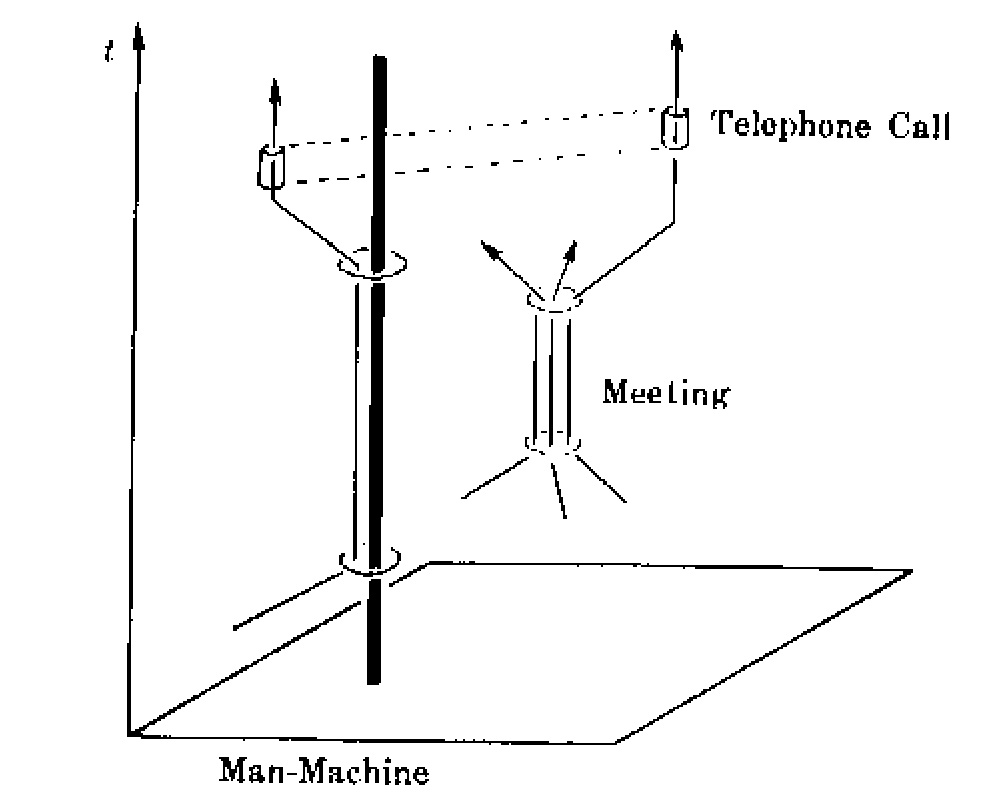
\includegraphics[width=0.9\textwidth]{figures/time-cube}
\end{center}
  \caption{Space-time prism, reproduced from \cite{Heagerstraand:1970ys}}
  \label{fig:prism}
\end{figure}

Instead of focusing on open ended possibilities, \citet{Heagerstraand:1970ys} instead chose to focus on the limits to an individual's freedom to move between places or perform activities  \citep[208]{10.2307/142726}. These were grouped into three constraints: capability constrains, which are limits to the available actions due to biology or tools, coupling constrains are limits due to the need to join with other individuals (or objects) to perform activities, authority constraints being those limits imposed by an authority. There is clearly a question as to whether cultures and societies studied archaeologically are subject to the same constraints, a premise of time-geography is that such constraints are universal and to truly benefit from it, this would have to be assumed. More challenging, perhaps, is the identification of evidence for the affects of such constraints. Time-geography focuses on hypothetical, rather than specific, individuals. It's advocates do not recommend following subjects around to create an inventory of how individuals spend their time, instead ``in choosing to develop a theoretical construct which reveals specific interactional and transactional constraints H{\"a}gerstraand is, in essence, rejecting any effort to directly predict individual behaviour'' \citep[210]{10.2307/142726}. Such a focus of analysis resonates with archaeological study, as it is not possible to trace the time-space path of specific individuals, but space and time as lived in and created by individuals is what is ultimately being studied, to put succinctly, it is the study of individuals, but not of an individual.

An area where time-geography could be particularly relevant to archaeology is simulation; in fact H{\"a}gerstraand himself suggested the use of simulation as analysis (until mathematical tools become available) \citep[21]{Heagerstraand:1970ys}. Simulation would particularly suit the idea of studying the constraints on individuals, in aggregate, or what \citet{10.2307/142726} calls the choreography of existence, it would also suit the second level of analysis, the physical existence of society, the pairing up between population and activity systems \citep[209]{10.2307/142726} and finally the prerequisite analysis required by \citet[214]{10.2307/142726} of singling out appropriate populations and applying aggregating procedures is less of a concern for a simulation as this can be included as part of the data generation step.

Returning to the focus of this chapter, the questions that can be asked of data, time-geography can be applied to understanding the constraints as identified by H{\"a}gerstraand, it can also examine how ideas, values, institutions, technology and natural rhythms interplay with the time-geographic routines of individuals and society as a whole \citep[213]{10.2307/142726}. Although it has been suggested that time-geography is not suited to the consideration of subjective constraints, psychological factors, cultural norms and social status \citep[218]{10.2307/142726} it is likely that some of these, specifically cultural norms and social status, will have some overlap with authority  and coupling constraints so need not be excluded altogether. The ideas of H{\"a}gerstraand have been developed in many different directions, of particular relevance to archaeology is the inclusion of phenomenological thinking, for example \citet{dur196} takes a two fold approach, firstly a sense of lived space-time drawing on the work of Merleau-Ponty and secondly by inclusion of the autonomous subject of Heidegger \citep[197]{dur196}. The result is a refashioned time-geography ``so that the paths retain the sense of expectation and memory suggested by Merleau-Ponty and Heidegger. A sense of space-time that brings the virtual into the experience of space, that thinks of space as connected to time'' \citep[206]{dur196} specifically focusing on the how past and future connect and are bound into the present and how ``Time is an experience of flow'' \citep[206]{dur196}. While the original concept of H{\"a}gerstraand involved a focusing on people, the inclusion of phenomenological thinking takes this one step further, to a sense of lived time-space. Another example of the combination of a social philosophy with time-geography is \citet{Pred1981-PREPEP} which overviews the concept of power with regard to social relations, attempts to conceptualise situations of power production, reproduction and transformation as part of a continual process of structuration, and portrays that process in terms of the continuous intersection of individual paths with institutional projects at specific temporal and spatial locations. The approach taken by \citet{Pred1981-PREPEP} while drawing heavily on social theory, is clearly rooted in the time-geographic tradition, placing the theory within the world of life-paths and constraints, dealing with the world as experienced by individuals, but not getting lost in the subjective experience or experience of a specific individual.

While the archaeological interest in phenomenology is extensive, the use of time-geography is much more limited and the two combined non-existent. Phenomenological thinking is not new to archaeology, however its application to time-geographic concepts presents many complications as well as opportunities when attempting to apply them to archaeological data. The study of the lived experience of time-geography surely is more than just the study of the experience of time-space as described by \citet{dur196}, a fundamental component must also be the lived experience of the constraints that are so central to time-geography. But experience is a fundamentally subjective factor and according to \citet[218]{10.2307/142726} such psychological, cultural or social constrains are excluded from the purview of time-geography. They would be challenging to study, with the focus of time-geography on exploring time-space through constraints on hypothetical individuals, but experience comes ultimately from a specific individual. Archaeologically the evidence for studying phenomenological experience is limited. \citet{fleming_2005} argues it is ``much more dependent on rhetoric, speculation, argument by assertion, and observations not always replicable when checked'' \citep[930]{fleming_2005}, and the evidence for the experience of time-space constraints is likely to be even more limited. However this does not mean that time-geography inspired studies should gloss over the fact that the constraints under study, and time-space itself are ultimately experienced by individuals.

The practical application of time-geography has focused heavily on planning contexts \citep[211]{10.2307/142726} and has been rarely applied to archaeological studies. In a recent attempt at integrating time-geographic techniques into archaeological analysis \citet{mlekuvz2010time} analysed travel times between two Roman towns using a cost surface analysis influenced by the constraints approach of time-geography. The study takes key capability constraints, such as the constraint that nobody can be in two places at the same time and that movement is time consuming as its time-geographic basis and constructs a space-time prism between the two towns, and makes an assumption of rational behaviour on the part of past agents. Ultimately the study created two models \citep[362]{mlekuvz2010time}, one of how accessible different parts of the landscape were from the location of known sites, within a given time budget and the other showing the number of points within a given time budget from which a location is accessible. The study is a very innovative method of combining the constraints of time-geography with a notion of the world as experienced in an archaeological context. Unfortunately it is purely speculative, no archaeological data is used in the process and the underlying assumption of (modern) rationality, while not entirely unreasonable without evidence to the contrary, is also unfounded. Crucially the resultant models are mostly influenced by the geographic structure of the landscape, the second model, entirely so. This assumes that the route choice is entirely driven by the environment, and is not altered by any joining or authority constraints, or any cultural factors. While mobility and movement are convenient means of attempting to understand the past as experienced, the results from the study are unfortunately highly speculative. In concluding \citep[364]{mlekuvz2010time} notes that ``time-geography does not come loaded with theoretical baggage'' which is surely a naive interpretation of a well established tradition of investigation and reasoning about people, the discussion above clearly demonstrates how different theoretical traditions have sought to adopt and influence time-geography in different directions, to adopt it uncritically is clearly a risky endeavour.

A second recent attempt at applying time-geography to archaeological data is \citet{doi:10.1559/152304009788988297} which is much more focused on the creation of software to display space-time prisms than it is on archaeological application or time-geographic concepts. Fundamentally it is a way of generating colourful (and confusing) diagrams, it does not consider time-geographic concepts, such as bundling or even constraints. The only representation of duration is on a site basis \citep[252]{doi:10.1559/152304009788988297}, as sites are static points in space (especially at a regional level) they need hardly have bothered presenting a diagram of the duration of site us in a space-time cube. The representation of duration is based on firm start and end dates, the tool is not capable of coping with one of the most common format of archaeological dates, the radiocarbon date. Fundamentally the tool does not consider people, and so is unrelated to time-geography in its entirety, it is barely capable of working with archaeological evidence and the analysis is based upon a comparison of pre-determined site attributes, which in this example are all environmental or geographic characteristics of the sites, such as slope, aspect, etc. Finally the available analytical procedures are limited and simplistic in nature. Clearly \citet{doi:10.1559/152304009788988297} have created a powerful tool, but one which was not designed with archaeological data in mind, while it has been influenced by time-geography it does not afford any analysis that is time-geographic and ultimately it does not consider people, a fundamental of time-geographic thought.

The influence of time-geography on archaeology has been more broad than the small number of studies attempting characteristically time-geographical analysis. It has also influenced interpretations more generally, such as \citet{barrett1994fragments} who considers the utilisation of time \citep[72]{barrett1994fragments} and interactions between people \citep[74]{barrett1994fragments} from a time-geographical perspective.

\section{Alternative Approach to Questions}
Having considered what are arguably the main approaches to temporal theory, it is now time to think about how this theory might be used to get the most out of spatio-temporal data. This must be more than simply taking the examples and time scales provided by others and applying them to new sites, as the questions asked must be applicable to the data available. In the same vein, there is also no need to be constrained, for example by only considering the four scales analysed by \citet{Bradley:2002fk}. Lucas clearly has this in mind when he states ``there is a lot more scope for exploring time in past societies, especially how it inflects with other social practices and concepts, such as power and gender'' \citep[118]{Lucas:2005fk}. He then suggests a potential line of inquiry ``to what extent did different sections of a prehistoric community experience time differently, and in association with what contexts?'' \citep[118]{Lucas:2005fk}. Lucas also suggests examining what he calls associated temporal concepts, such as remembering and forgetting, old and new, continuity and change \citep[94]{Lucas:2005fk}, again these are only examples, what is in many ways more significant is that there is clearly plenty of opportunity for exploring time. That such questions about society can be answered with the aid of computational methods is demonstrated by certain spatial studies, for example \citet{Kosiba:2013fk} used GIS methods to explore how social differences are embedded in spatial boundaries in the Inka empire. Using primarily visibility analysis they were able to determine restricted, exclusive ceremonial, and residential areas, \citep[93]{Kosiba:2013fk} and turned the identified spatial boundaries into social ones, thus developing an understanding of how the social perception and experience was shaped by political forces \citep[94]{Kosiba:2013fk}.

From the perspective of an individual site, there is clearly plenty of potential to examine the changes between key phases of use, for example at Hambledon it may be possible to consider how the Mesolithic use related to the Neolithic uses. During the Neolithic the site was used intermittently \citep[755]{Mercer:2008fk}, which provides a great deal of scope for spatio-temporal analysis, in particular, were the same parts of site used together, or is there evidence for a change in the locus of use over time? Does the usage appear to be the same over a long period, and can this suggest a continuity of belief? Could the site be seen as a tool for maintaining social protocols over a period of time? The excavator suggests the use may have been infrequent \citep[755]{Mercer:2008fk} in which case might each event have required a reinterpretation of the site, of the physical remains that were found and re-worked at each event? Each period of use would surely have been influenced by those remains from the past that were extant at the time. Along a similar vein, episodes of re-digging of ditches would likely result in deposited material from the past being excavated, although clearly the finding of articulated remains demonstrates that some areas were not re-dug, possibly by chance, or maybe due to the memory of their location, potentially aided by physical reminders, \citep[759]{Mercer:2008fk}. In fact, the excavator does suggest that the uses of particular ditch segments were remembered with the same type of use occurring over a long period of time \citep[756]{Mercer:2008fk}. 

There is also the potential to consider multiple timescales, from the short-term events, to the longer scale of monument construction and Hambledon's place in social networks. Clearly there are opportunities for exploring long term processes, such as repeated re-use of particular areas, also the suggestion from the excavator that the more defensive elements were potentially built to follow a plan of some sort \citep[760]{Mercer:2008fk}. It also might only be over longer time frames that the changes to areas that are a focus for use become apparent, with such drift, or relocation of activity hidden by noise at a smaller scale. Finally it may be possible to consider how use in the later phases was influenced by the remains of much earlier activity, in particular the excavators assertion that the enclosure was recognised, and used, into the second millennium BC \citep[770]{Mercer:2008fk}. However, at some point subsequent to that, it was disregarded, and by the Iron Age, there was a field system laid out as though earlier earthworks no longer existed \citep[770]{Mercer:2008fk}.

From a larger spatial perspective the Gathering Time project \citep{Whittle:2011kl,Whittle:2011tg} offers the ability to consider similar site-level questions, but across multiple sites and a comparison of the answers. At the inter-site level, similar questions could be asked of landscapes, such as how existing monuments affect the building of new monuments, both of the same type and of entirely different types. In addition monuments need not be considered a totality, depending on the resolution of the temporal data it may be possible to analyse the spatial dimension of the alteration of sites, for example do particular alterations happen within a constrained timeframe across sites in a particular locality.

Finally, at a national, or inter-national level there is the potential to not only examine larger processes, but also tie these back down to local phenomena, for example Bradley's potential link between long house orientation, and the notion of ancestral homelands. There is an enormous amount of scope at this layer for a wide variety of potential lines of inquiry, other examples could include, taking current spatio-temporal approaches on the spread of the Neolithic, and examining notions of past and identity, how did incoming people or ideas affect a populations view of its own past, its traditions and heritage. \citet{BocquetAppel2009807} identified that the process was not smooth, so during the periods of pause, and then subsequent rapid spread, how did that affect notions of the past? Presumably if pauses lasted for generations the new ideas or new people would become incumbent, a part of the status quo and the inherited past in these areas would be different (at least at first) from that of areas of rapid change. A recent example of such a study is \citet{whittle2018times} which considers a range of themes and sites across Europe and at different scales of time.

This chapter has considered both routine and more theory driven approaches to the questions that have been asked of archaeological remains. Specifically, but not exclusively, temporal questions, how such questions can trivially be extended into the spatial domain and some hypothetical lines of enquiry. Next, we will consider the kind of methods that can analyse the archaeological remains, or raw data. The analysis will be used to take a step towards answering questions that go beyond the descriptive.